\documentclass[11pt,a4paper,utf8x]{report}
\usepackage[T1]{fontenc} 
\usepackage[utf8x]{inputenc}  
\usepackage{lmodern}
\usepackage [frenchb]{babel}

% Pour pouvoir utiliser 
\usepackage{ucs}

\usepackage{textcomp}
\usepackage{graphicx}
\usepackage{keystroke}
\usepackage{amssymb}
\usepackage{amsmath}
\renewcommand{\thesection}{\arabic{section}} % numérotation des sectiosn
\usepackage[cc]{titlepic} %rajouter le logo dans la page de garde
\usepackage{url} % Pour avoir de belles url
\usepackage {geometry}
\usepackage[linktocpage]{hyperref}

% Pour mettre du code source
\usepackage {listings}
% Pour pouvoir passer en paysage
\usepackage{lscape}	

% Pour pouvoir faire plusieurs colonnes
\usepackage {multicol}

% POur crééer un index
\usepackage{makeidx}

\usepackage{graphicx}

\hypersetup{
colorlinks=true, %colorise les liens
breaklinks=true, %permet le retour à la ligne dans les liens trop longs
urlcolor= blue, %couleur des hyperliens
citecolor=	cyan,
bookmarksopen=true,
%si les signets Acrobat sont créés,
%les afficher complètement.
pdftitle={\'Etude algorithmique}, %informations apparaissant dans
pdfauthor={MARGUERITE Alain\\ RINC\'E Romain},
%dans les informations du document
pdfsubject={Doc}
%sous Acrobat.
}
\makeindex

\title{\'Etude algorithmique}
\titlepic{
\includegraphics[scale=0.80]{img/logolina}     \hspace{2cm} 
\includegraphics[scale=0.80]{img/logouniv}}


\author{MARGUERITE Alain\\ RINC\'E Romain}
\date{Université de Nantes \\ 2 rue de la Houssinière, BP92208, F-44322 Nantes cedex 03, FRANCE}

\begin{document}

\maketitle
\clearpage

\tableofcontents
\clearpage
\section{Stockage des boites et visualisation}
Trois problèmes majeurs apparaissent dans la réalisation du logiciel de visualisation. La première est bien entendu la gestion d'une très grande quantité de boites lors de l'affichage. Il est en effet nécessaire d'offrir un accès rapide au informations des boites dans la fenêtre. La seconde est la gestion des filtres sur ces mêmes boites. Et le troisième apparait lors du changement des variables étudiées (changement des dimensions visualisées).

\subsection{\'Etude d'une solution possible : le Quadtree}
\paragraph{}Une des solutions qui permettrait d'offrir une visualisation fluide du pavage en permettant aisément de répondre au cahier des spécifications serait de représenter le pavages sous une forme de quadtree pour deux dimensions ou octree pour trois dimensions.

\paragraph{Le quadtree}consiste à découper un espace fini en deux dimensions en quatre parties égales chacune étant stocker dans un nœud ; puis on itère ce mécanisme sur chacun de ces nœuds jusqu'à isolé spatialement les éléments recherchés.
\begin{figure}[htbp]
\centering
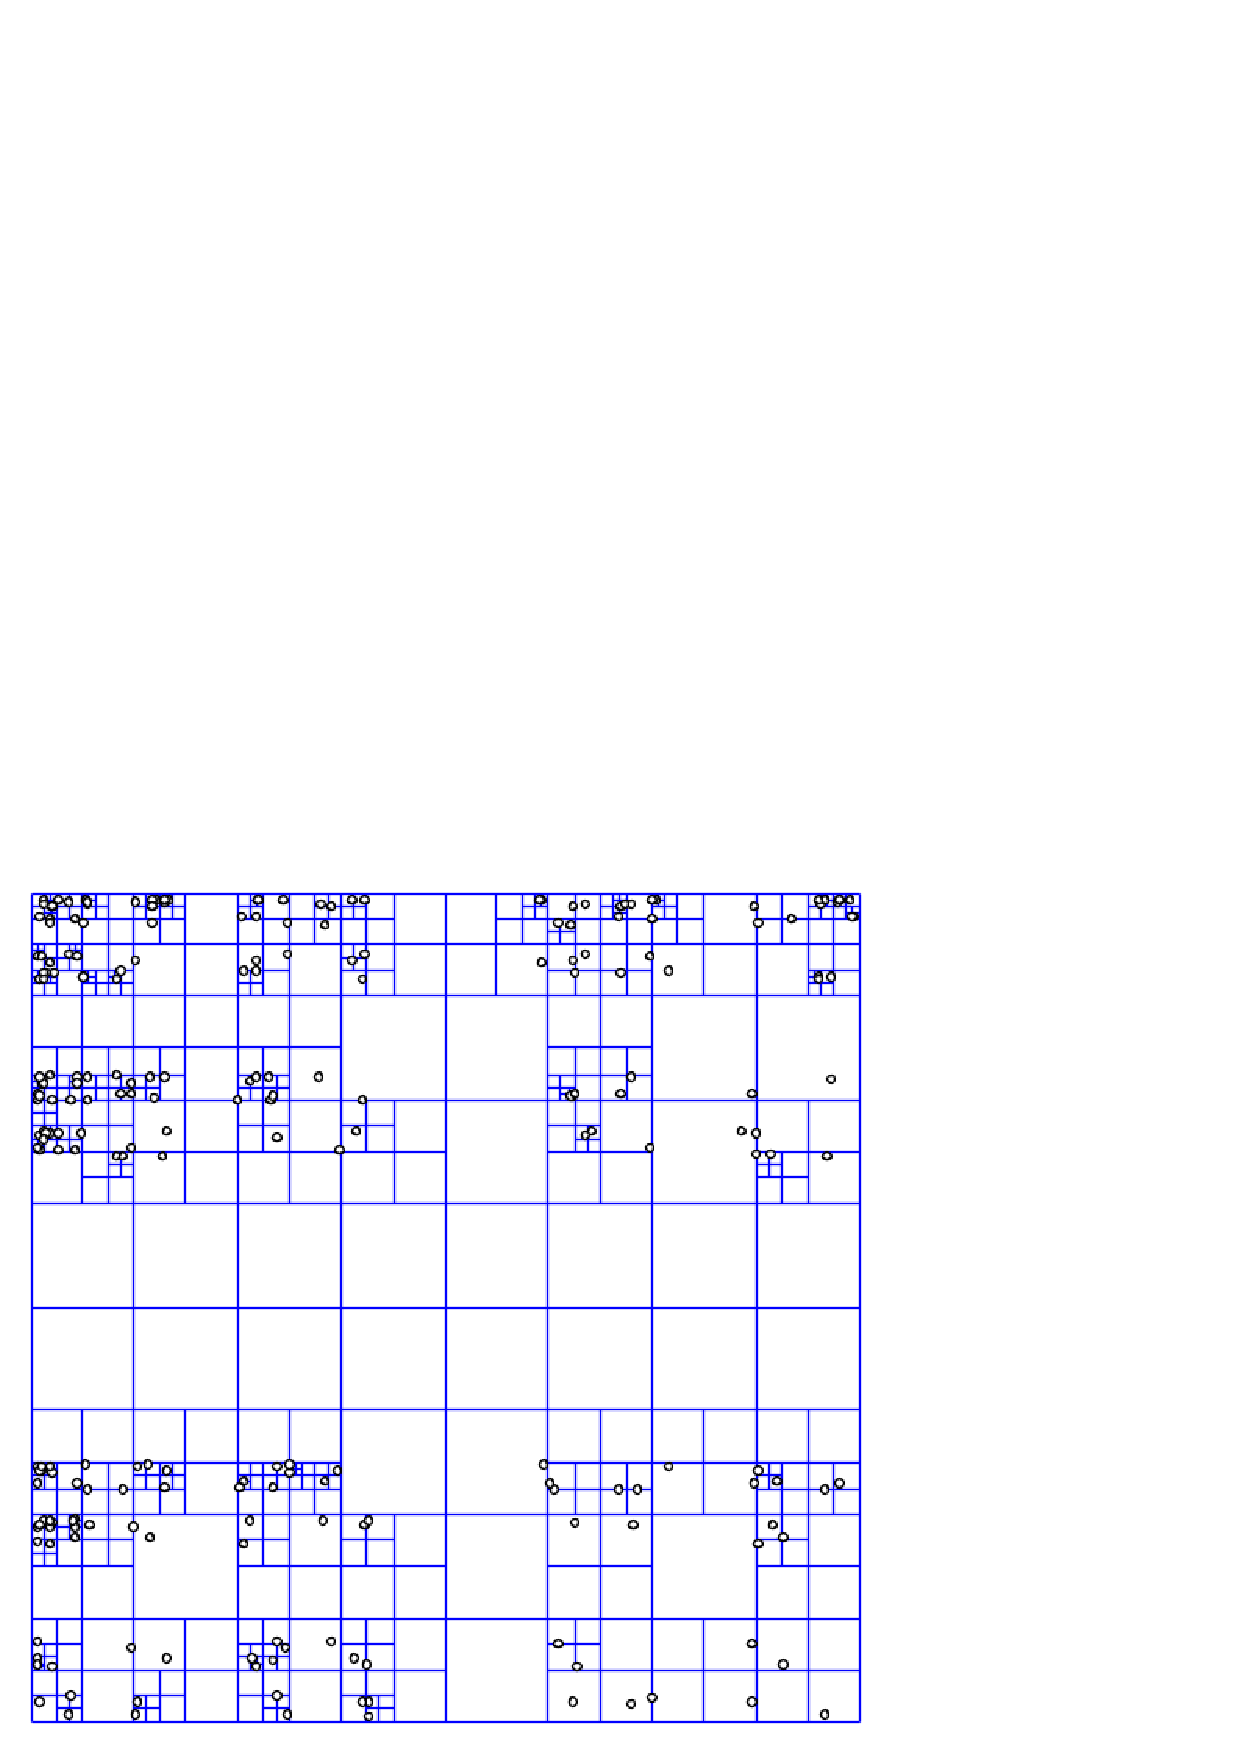
\includegraphics[scale=0.50]{quadtree}
\caption{Représentation d'un quadtree}
\end{figure}
Cette strucure pourrait être utilisé pour déterminer la position des boites dans l'espace selon la méthode suivante :
\begin{itemize}
\item Si un des nœuds du quadtree ne contient aucune boite ou qu'il est entièrement inclus dans un ensemble de boites alors il n'est plus nécessaire de le subdiviser. Ce nœud contiendra donc une référence sur chacune de ces boites.
\item \`A contrario si un nœud du quatree contient une des bornes d'une des boites, alors il est nécessaire de subdiviser ce nœud.
\item On arrête aussi de diviser les nœuds lorsque l'on arrive à une précision inférieur à la précision du calcul de Realpaver.
\end{itemize}

L'octree repose sur le même principe mais étendu à trois dimensions. L'espace est donc découpé en huit parties à chaque fois.

Cette structure est particulièrement intéressante pour la visualisation du pavage. En effet pour une fenêtre de visualisation donnée, il est très simple et rapide d'extraire la sous-arborescence correspondante à l'espace visualisé et permet aussi de ne pas afficher les objets trop petits.

Le problème de cette méthode est essentiellement à la construction puisque la structure devra découper en la plus petite feuille possible au niveau des bornes des boites ce qui va nécessairement entrainer la construction d'un grand nombre de feuilles. Ce problème est particulièrement gênant puisque si l'on cherche à localiser une boite de dimensions 1 sur 1 avec la précision donnée par défaut par Realpaver de $10^{-16}$, on se retrouve avec au moins $4 \times 10^{16}$ feuilles. On peut optimiser l'algorithme de construction en considérant que si un des nœuds contient l'intégralité ou une partie d'une seule boite, il n'est plus nécessaire de subdiviser, la recherche d'une seule boite étant immédiate.

Un autre problème apparait lorsque l'utilisateur souhaite changer les variables visualisées dans l'outil. Si l'on reste sur une structure en du type quadtree ou octree, il sera nécessaire de recalculer entièrement l'arbre.

On pourrait alors supposer une structure similaire $k$-dimensionnelle\footnote{$k$ étant la dimension du problème fourni à Realpaver.} où chaque nœud possède $2^k$ nœuds. L'avantage d'une telle structure est que lorsque l'on désire changer les variables de visualisation, le calcul est déjà effectué.

\paragraph{} Malgré le fait que le quadtree pouvait être une structure intéressante, le nombre de feuilles créées est bien trop important et ne peut donc pas être utilisé.

\subsection{\'Etude d'une seconde solution : le R-tree}
\paragraph{Le R-tree} est une structure de données utilisée pour stocker des informations $k$-dimensionnelles. Le principe est le suivant :
\begin{itemize}
 \item Un noeud de l'arbre correspond à une boite non-solution du pavage.
 \item Chaqu e boite peut contenir entre $m$ et $M$ sous-boites entièrement incluses. Avec $m\leq \frac{M}{2}$.
 \item Une feuille de l'arbre est une boite ne contenant que des boites solution du pavage.
 \item L'arbre est équilibré.
\end{itemize}

La figure \ref{fig:rtree} donne une bonne idée du principe des R-trees\cite{wiki}:
\begin{figure}[htbp]
\centering
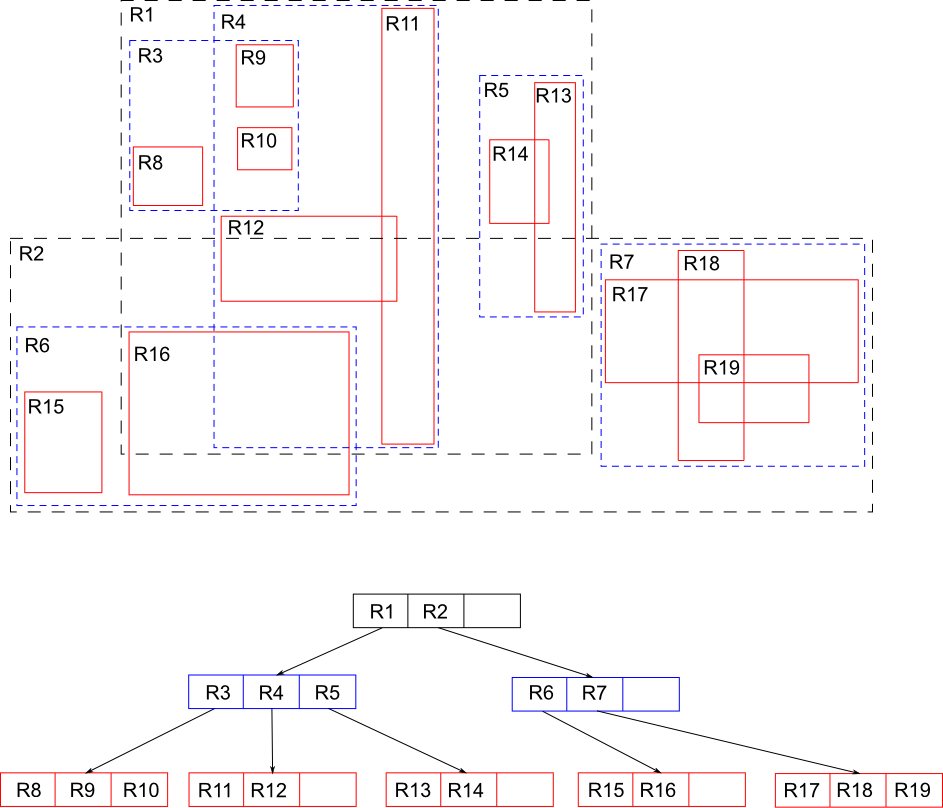
\includegraphics[scale=0.50]{rtree}
\caption{Représentation d'un R-tree}
\label{fig:rtree}
\end{figure}

Pour plus de détails sur le R-tree on pourra se référer à l'article de A. Guttman \cite{Guttman}

\paragraph{} Une telle structure semble bien plus intéréssante en terme d'occupation mémoire. En effet le nombre de feuilles de l'arbre est au pire égale à $\frac{N}{m}$. Cependant on peut se demander si rechercher une fenêtre de visualisation sera efficace. En effet il est nécessaire de parcourir toutes les boites dont l'intersection est non nulle avec la fenêtre. De nombreuses analyses ont été effectuées sur le sujet. On pourra se reporter sur une analyse de performances sur les Priority R-trees \cite{PRTree}.
\appendix
\bibliographystyle{alpha}
\bibliography{source.bib}

\end{document}
